\section{Applications of Differentiation}

\subsection{Extrema: Maxima and Minima}

This leads us to a very important application of calculus showing the existence of and finding extrema. That is, finding the points at which functions attain their extrema i.e. their maxima or minima.

\begin{defn}
  We say that $f$ has a \emph{local maximum} at $c$ if
  \[
f(c)\geq f(x)\ \text{for all }x\text{ sufficiently close to } c.
  \]
Likewise, we define the \emph{global maximum of $f$} to be the point $c$ such that
\[
f(c)\geq f(x)\ \text{for all }x\text{ where $f$ is defined.}
\]
We can define local and global minima similarly by flipping the inequality.
\end{defn}

One thing to notice is that not all functions have local extrema. For example, take the function
\[
f(x)=x \text{ where } 0<x<1
\] or
\[
f(x)= \begin{cases}
0 \text{ when $x$ is in } \bbQ,  \\
1 \text{ otherwise},
\end{cases}
\] which has no local maxima or minima though every point is an absolute maximum or minimum. Luckily, the Extreme Value Theorem gives us criteria to tell when a function has absolute extrema.

\begin{thm}[Extreme Value Theorem]
  If $f$ is continuous on a closed interval $[a,b]$, then $f$ has both a global maximum and minimum on that interval.
\end{thm}

This gives us a neat answer in the case $f$ is continuous on a closed interval $[a,b]$, but what happens if we further assume that $f$ is differentiable on the open interval $(a,b)$.


Let's consider the function $f(x)=1-x^2$ on the interval $[-1,1]$. Clearly, $f$ is continuous on $[-1,1]$ and differentiable on $(-1,1)$. By the Extreme Value Theorem, you can see that we're guaranteed a maximum and minimum on $[-1,1]$. Graphing the function, we see that the minimum occurs at $x=1,-1$ where $f(x)=0$ and that the maximum occurs at $x=0$ where $f(x)=1$. Let's see what this entails for the derivative of $f$. \\


The derivative of $f(x)$ is $f'(x)=-2x$. From this, we can notice that if $x<0$, then $f'(x)>0$. That is $f(x)$ has a positive slope to its tangent and is \emph{increasing}. Similarly, when $x>0$, $f'(x)<0$ and $f$ is \emph{decreasing}.  Furthermore, $f'(0)=0$ which makes sense since for $f$ to achieve a maximum at 0, it must increase to a point and then decrease from there on for $x$ near 0. This means that not only does $f$ have a global maximum at 0; it also has a local maximum.

%% Graph function above show the tangent line for a decreasing and increasing point and a third at minimum.


Above we used the sign of the derivative $f'$ to determine whether $f$ was increasing or decreasing. In general, this holds for every differentiable function $f$.

\begin{prop}
Given a differentiable function $f$,
\begin{enumerate}
  \item If $f'(x)>0$, then $f$ is increasing at $x$.
  \item If $f'(x)>0$, then $f$ is decreasing at $x$.
\end{enumerate}
\end{prop}

This leaves us to understand the case where $f'(x)=0$. We can begin to describe this case using what is known as the \emph{first derivative test}.

\begin{thm}[First Derivative Test]

\end{thm}

%% Make sure to use the language of stationary and critical points


%% Give example of a function with maximum. Then state that $f'(c)$ must be 0.


%% Use as justification for stating how derivative must change from positive to negative! i.e. first derivative test.

%% State second derivative test.

\subsection{Optimization}

%% General Idea, Examples, hint at Calculus of Variations

%% Use the ellipse example for calculus of variations blog post!

\subsection{Linear Approximations}

By construction, the derivative describes the instantaneous rate of change of a function at a particular point. As we saw, this is the slope of the tangent line at that point. Because of this, the derivative can be used to provide an estimate of what the function is doing near a given points. That is, if we fix a function $f$ and a point $a$ where $f$ is differentible, we can use the derivative $f'(a)$ and its corresponding tangent line to $f$ to approximate the function $f$ at points $x$ near $a$. This process is called \emph{linear approximation}.

%% Lay out the statement and do examples where computing might be hard, compare error.

%% Talk about Euler's method (or Newton's method idk which one it is)... direct towards the will be appendix
\subsection{Implicit Differentiation}

In the cases given previously, we have always been able to isolate our expressions as functions of single variable i.e
\[
f(x)=x^2+5x-3\text{ or }y=\frac{\sin (x+1)}{x^2}.
\]
This may not always be possible or the simplest way to do things! Suppose we're given the equation for a circle centered at the origin with radius 1

\[
x^2+y^2=1.
\]

Yes, it is possible to isolate $y$ and find $y=\pm \sqrt{1-x^2}$, but this leaves two different cases to watch out for when finding the derivative on the circle.\\

Instead, if we remember that $y$ is a function as $x$, we can differentiate this equation without isolating $y$ using the \emph{chain rule} as follows:
\begin{equation}
  \diff{}{x}\big[x^2+y^2=1\big]\implies 2x+2y\diff{y}{x}=0.
\end{equation}
Rearranging this, we see that
\[
\diff{y}{x}=-\frac{x}{y} \text{ where $x,y$ satisfy the equation we started with.}
\]

This technique is called \emph{implicit differentiation} and comes in handy when dealing with complex expressions in terms of both $y$ and $x$. Let's do another example.

\begin{exmp}
  Let's consider the curve given by
\begin{equation}\label{ImplicitFunc1}
  y^3-y = x^3-x\cos(30x).
\end{equation}

Suppose we wanted to find the slope of a point tangent to this curve. Instead of hopelessly trying to simplify this equation to solve for $y$ and differentiate, we can differentiate implicitly. Differentiating \eqref{ImplicitFunc1} with respect to $x$, we get \[
3y^2\diff{y}{x}-\diff{y}{x}=3x^2-\cos(30x)-30x\sin(30x).
\]
Pulling out the $\diff{y}{x}$, we see
\[
\diff{y}{x}=\frac{3x^2-\cos(30x)+30x\sin(30x)}{3y^2-1}.
\]
Notice that this derivative is undefined along the lines $y=\pm\frac{1}{\sqrt{3}}$, which correspond the points where the line tangent to the graph is vertical. Similarly, we can find the points where the slope is horizontal by finding the zeroes of $3x^2-\cos(30x)+30x\sin(30x)$.


\begin{figure}
  \centering
  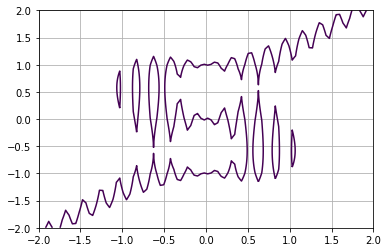
\includegraphics[width=0.4\linewidth]{ImplicitFunc1.png}
  \caption{Graph of (\ref{ImplicitFunc1})}
\end{figure}
\end{exmp}

We can can use implicit differentiation to prove \cref{SinCosExpDif}.3. using \cref{SinCosExpDif}.4.  i.e. that derivative of $f(x)=e^x$ is $e^x$.
\begin{proof}
Suppose we have $y=e^x$. This is equivalent to saying that $\ln y = x$.
Taking the derivative of both sides with respect to $x$, we see that
\[
\frac{1}{y}\diff{y}{x}=1,
\]
using that $\diff{}{y}\left( \ln y \right) = \frac{1}{y}$. Therefoere,
$\diff{y}{x}=y=e^x$.
\end{proof}

\begin{exer}
  Prove that $\diff{}{x}\left( \ln x \right) = \frac{1}{x}$ using that the derivative of $e^x$ is itself.
\end{exer}

\subsection{Related Rates}
